\section{Højtaleren i Lukket Kabinet}

Sammenholdt med teorien for det lukkede kabinet i afsnit \ref{chapt:Teori}, kan frekvensrepsonset for projektets højtalenhed simuleres i matlab, som det ses på figur \ref{fig:simLukketKab}, ved en antagelse om at kabinettet udgør en uendelig baffel, og der dermed ikke er nogen påvirkning af kantdifraktion, refleksion eller tab igennem kabinettet.  
Det kan noteres, at under resonansfrekvensen på 65 Hz, falder kurven fast med ca. 12 dB/oktav, og har ikke noget overshoot som peak, som det kan ses gøre sig gældende i næste afsnit for basreflekskabinettet. 


\begin{figure}[h!]
	\centering
	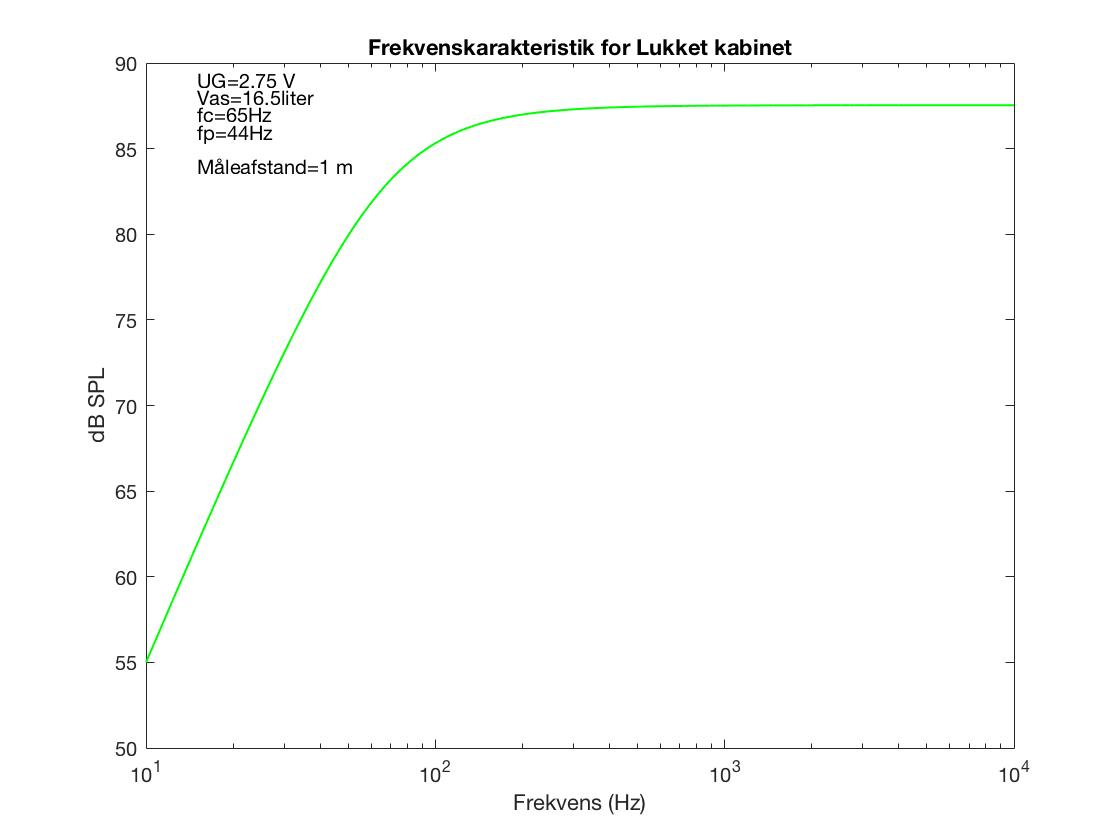
\includegraphics[width=.8\textwidth]{Pics/simLukketKab}
	\caption{frekvensrepsons for Højtalerenheden i lukket kabinet } 
	\label{fig:simLukketKab}
\end{figure}

Yderligere beregningsparametre omtales i næste afsnit, omhandlende projektets fokuskabinet: basrefleks-kabinettet. 


